
\documentclass[11pt,a4paper]{article}
\usepackage[margin=1.7cm]{geometry}
\usepackage{amsmath,amssymb}
\usepackage{tikz}
\usepackage{xcolor}
\usepackage{parskip}
\usepackage[T1]{fontenc}
\usepackage[utf8]{inputenc}
\usepackage[dutch]{babel}
\usepackage{newtxtext,newtxmath}
\usetikzlibrary{arrows.meta,calc,positioning,decorations.pathmorphing}

\setlength{\parskip}{0.55em}
\setlength{\parindent}{0pt}

\newcommand{\uncertain}[1]{\textit{\textcolor{gray}{#1}}}

\title{Notebook 2012 --- Pagina's 52, 54 en 55}
\author{}
\date{}

\begin{document}
\maketitle

\uncertain{Pagina 53 is op verzoek overgeslagen. De schetsen zijn geometrisch genormaliseerd, maar volgen de oorspronkelijke kleurcodering en structuur zo dicht mogelijk. Onduidelijke woorden en symbolen zijn als onzeker gemarkeerd.}

\clearpage
\section*{Pagina 52}

\begin{minipage}[t]{0.48\textwidth}
\subsection*{Linkerhelft}

\begin{center}
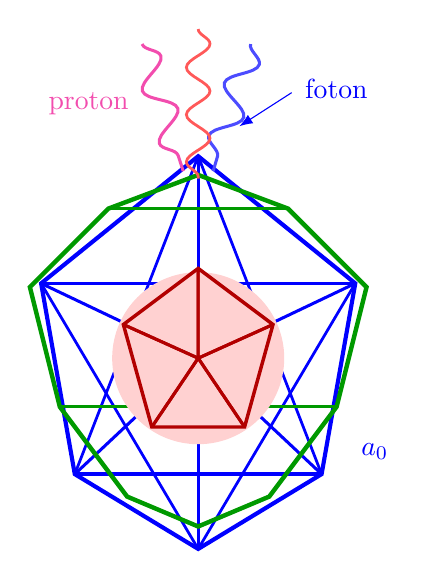
\begin{tikzpicture}[scale=0.95,>=Latex]
    % outer projected icosahedron
    \coordinate (T) at (0,2.7);
    \coordinate (UL) at (-2.1,1.0);
    \coordinate (UR) at (2.1,1.0);
    \coordinate (LL) at (-1.65,-1.55);
    \coordinate (LR) at (1.65,-1.55);
    \coordinate (B) at (0,-2.55);
    \coordinate (C) at (0,0);

    \draw[blue, line width=1.5pt] (T)--(UL)--(LL)--(B)--(LR)--(UR)--cycle;
    \draw[blue, line width=1.25pt] (UL)--(UR);
    \draw[blue, line width=1.25pt] (LL)--(LR);
    \draw[blue, line width=1.1pt] (T)--(C)--(B);
    \draw[blue, line width=1.1pt] (UL)--(C)--(UR);
    \draw[blue, line width=1.1pt] (LL)--(C)--(LR);
    \draw[blue, line width=1.0pt] (T)--(LL);
    \draw[blue, line width=1.0pt] (T)--(LR);
    \draw[blue, line width=1.0pt] (B)--(UL);
    \draw[blue, line width=1.0pt] (B)--(UR);

    % green dodecahedral envelope
    \draw[green!60!black, line width=1.6pt]
      (-2.25,0.95)--(-1.2,2.0)--(0,2.45)--(1.2,2.0)--(2.25,0.95)
      --(1.85,-0.65)--(0.95,-1.85)--(0,-2.25)--(-0.95,-1.85)
      --(-1.85,-0.65)--cycle;
    \draw[green!60!black, line width=1.1pt] (-1.2,2.0)--(1.2,2.0);
    \draw[green!60!black, line width=1.1pt] (-1.85,-0.65)--(1.85,-0.65);

    % central proton/polyhedron
    \fill[red!18] (0,0) circle (1.15);
    \draw[red!70!black, line width=1.25pt] (0,1.2)--(-1.0,0.45)--(-0.62,-0.92)--(0.62,-0.92)--(1.0,0.45)--cycle;
    \draw[red!70!black, line width=1.1pt] (0,1.2)--(0,0)--(-1.0,0.45);
    \draw[red!70!black, line width=1.1pt] (0,1.2)--(0,0)--(1.0,0.45);
    \draw[red!70!black, line width=1.1pt] (-1.0,0.45)--(0,0)--(-0.62,-0.92);
    \draw[red!70!black, line width=1.1pt] (1.0,0.45)--(0,0)--(0.62,-0.92);
    \draw[red!70!black, line width=1.1pt] (-0.62,-0.92)--(0,0)--(0.62,-0.92);

    % photon-like intertwined trajectories
    \draw[magenta!70, line width=1.1pt, decorate, decoration={snake, amplitude=1.8mm, segment length=7mm}]
      (-0.75,4.2) -- (-0.2,2.5);
    \draw[blue!70, line width=1.1pt, decorate, decoration={snake, amplitude=1.8mm, segment length=7mm}]
      (0.7,4.2) -- (0.2,2.5);
    \draw[red!65, line width=1.0pt, decorate, decoration={snake, amplitude=1.5mm, segment length=6mm}]
      (0,4.4) -- (0,2.4);

    \node[blue, right] at (1.3,3.6) {foton};
    \draw[blue,->] (1.25,3.55) -- (0.55,3.1);
    \node[magenta!70, left] at (-0.8,3.4) {proton};
    \node[blue, right] at (2.05,-1.25) {$a_0$};
\end{tikzpicture}
\end{center}

\begin{align*}
20 &\quad \text{icosahedron}
\\
12 &\quad \text{dodecahedron}
\end{align*}

\uncertain{Onderaan staan de labels ``ground ball'' en ``proton''.}
\end{minipage}
\hfill
\begin{minipage}[t]{0.48\textwidth}
\subsection*{Rechterhelft}

\begin{center}
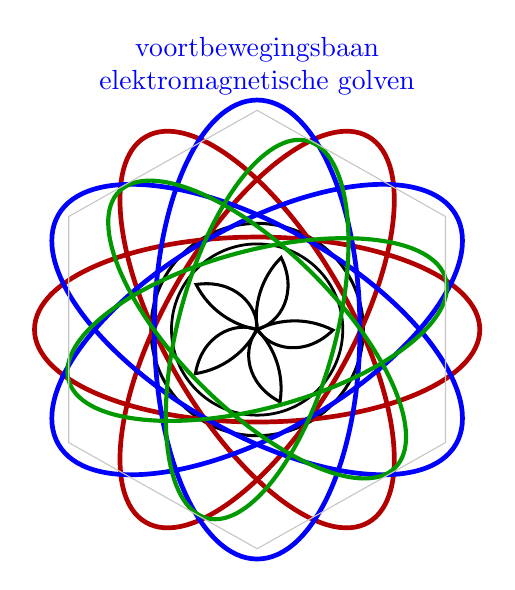
\begin{tikzpicture}[scale=0.87,>=Latex]
    % central flower
    \foreach \a in {0,72,144,216,288}{
        \begin{scope}[rotate=\a]
        \draw[black, line width=1.1pt] (0,0)
            .. controls (0.35,0.1) and (0.6,0.55) .. (0.35,1.05)
            .. controls (0.05,0.75) and (-0.05,0.35) .. (0,0);
        \end{scope}
    }
    \draw[black, line width=1.0pt] (0,0) circle (1.25);
    \draw[black, line width=1.1pt] (0,0) circle (1.55);

    % orbital / EM loops
    \foreach \angle in {0,60,120}{
        \begin{scope}[rotate=\angle]
            \draw[red!70!black, line width=1.7pt] (0,0) ellipse (3.25 and 1.35);
        \end{scope}
    }
    \foreach \angle in {30,90,150}{
        \begin{scope}[rotate=\angle]
            \draw[blue, line width=1.7pt] (0,0) ellipse (3.35 and 1.5);
        \end{scope}
    }
    \foreach \angle in {15,75,135}{
        \begin{scope}[rotate=\angle]
            \draw[green!60!black, line width=1.5pt] (0,0) ellipse (2.85 and 1.15);
        \end{scope}
    }

    % faint construction polygon
    \draw[gray!45] (0,3.2)--(2.75,1.65)--(2.75,-1.65)--(0,-3.2)--(-2.75,-1.65)--(-2.75,1.65)--cycle;

    \node[blue, align=center] at (0,3.85)
      {voortbewegingsbaan\\elektromagnetische golven};
\end{tikzpicture}
\end{center}

oneindige constructieve\\
golfinterferentie\\
met Fibonacci?

\uncertain{De titel boven het diagram is gedeeltelijk onzeker; ``voortbewegingsbaan elektromagnetische golven'' is de meest waarschijnlijke lezing.}
\end{minipage}

\clearpage
\section*{Pagina 54}

\begin{minipage}[t]{0.49\textwidth}
\subsection*{Linkerhelft}

Vanaf elk punt ontvang je een straal\\
licht uit links en rechts.

\[
\text{Universum is een 6-dimensionale torus}
\]

\begin{align*}
V_6 &= \frac{16\pi^3}{15}\,r^6
\\
    &= 33{,}0733508\,r^6
\end{align*}

\[
2(3+1)\text{-dimensionale torus}
\]

{\color{green!50!black}
\[
V_x
=
\frac{\Gamma}{2\pi D}
\left[
\ln\left(\frac{4D}{r}\right)-\frac14
\right]
\]
}

\begin{center}
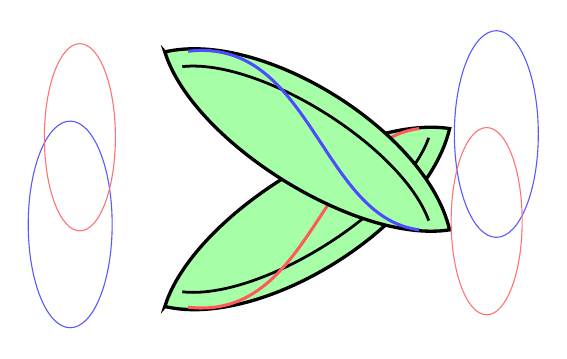
\begin{tikzpicture}[scale=0.82,>=Latex]
    % linked torus ribbons
    \begin{scope}[rotate=32]
      \draw[black, line width=1.2pt, fill=green!35]
        (-2.6,-0.7) .. controls (-1.5,-1.8) and (1.5,-1.8) .. (2.6,-0.7)
        .. controls (1.5,0.25) and (-1.5,0.25) .. cycle;
      \draw[black, line width=1.0pt]
        (-2.25,-0.65) .. controls (-1.3,-1.4) and (1.3,-1.4) .. (2.25,-0.65);
      \draw[red!65, line width=1.1pt]
        (-2.3,-0.9) .. controls (-0.8,-2.1) and (0.8,0.2) .. (2.2,-0.45);
    \end{scope}

    \begin{scope}[rotate=-32]
      \draw[black, line width=1.2pt, fill=green!35]
        (-2.6,0.7) .. controls (-1.5,1.8) and (1.5,1.8) .. (2.6,0.7)
        .. controls (1.5,-0.25) and (-1.5,-0.25) .. cycle;
      \draw[black, line width=1.0pt]
        (-2.25,0.65) .. controls (-1.3,1.4) and (1.3,1.4) .. (2.25,0.65);
      \draw[blue!70, line width=1.1pt]
        (-2.3,0.9) .. controls (-0.8,2.1) and (0.8,-0.2) .. (2.2,0.45);
    \end{scope}

    \draw[blue!65] (-3.3,-0.7) ellipse (0.65 and 1.6);
    \draw[blue!65] (3.3,0.7) ellipse (0.65 and 1.6);
    \draw[red!55] (-3.15,0.65) ellipse (0.55 and 1.45);
    \draw[red!55] (3.15,-0.65) ellipse (0.55 and 1.45);
\end{tikzpicture}
\end{center}

\[
2\cdot3+1=7
\]

{\color{green!50!black}
1 dimensie tijd om de vortex te maken
}

\end{minipage}
\hfill
\begin{minipage}[t]{0.47\textwidth}
\subsection*{Rechterhelft}

{\color{green!50!black}\textbf{di Bartini}}
\qquad
\[
2N+1=\pm 7
\]

{\color{green!50!black}
Vond de meest waarschijnlijke\\
formatie voor een vortextorus.

Bij de $2N+1=\pm7$ vond\\
hij extreme antwoorden.
}

\begin{align*}
E_1
&=
\frac{D}{r}
=
\frac14 e^{6{,}9996468}
\\
&\approx 274{,}074996
\end{align*}

\begin{align*}
R &= \frac12 D
\\
\frac{274{,}074996}{2}
&=
137{,}037498
\end{align*}

\begin{align*}
v
&=
c\frac{r}{R}
=
\frac{2c}{E_1}
\\
&\approx
2{,}1876\cdot10^6\ \mathrm{m\,s^{-1}}
\\
&\approx 2v_e
\end{align*}

\uncertain{Het eerste symbool in de verhouding $E_1=D/r$ kan ook als een andere hoofdletter zijn bedoeld. De numerieke waarden zijn goed leesbaar.}
\end{minipage}

\clearpage
\section*{Pagina 55}

\begin{minipage}[t]{0.48\textwidth}
\subsection*{Linkerhelft}

\begin{center}
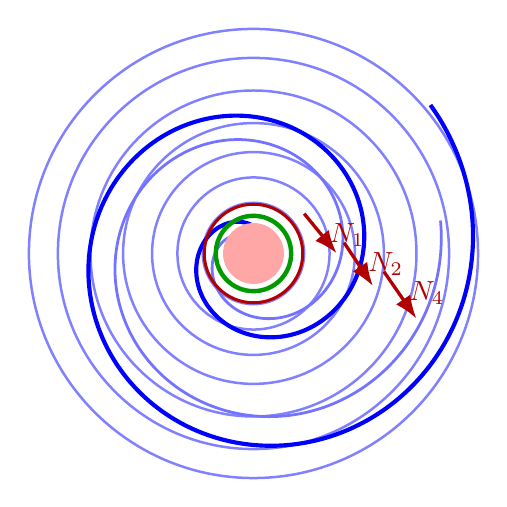
\begin{tikzpicture}[scale=0.92,>=Latex]
    % outer vortex rings
    \foreach \r in {0.7,1.05,1.4,1.8,2.25,2.7,3.1}{
      \draw[blue!70, opacity=0.7, line width=0.9pt] (0,0) circle (\r);
    }

    % spiral swirl
    \draw[blue, line width=1.5pt]
      plot[domain=0:760,samples=240,smooth,variable=\t]
      ({0.0042*\t*cos(\t)}, {0.0042*\t*sin(\t)});

    \draw[blue!55, line width=1.0pt]
      plot[domain=0:690,samples=220,smooth,variable=\t]
      ({0.0038*\t*cos(\t+40)}, {0.0038*\t*sin(\t+40)});

    % core
    \fill[red!35] (0,0) circle (0.42);
    \draw[green!60!black, line width=1.6pt] (0,0) circle (0.52);
    \draw[red!70!black, line width=1.1pt] (0,0) circle (0.68);

    % arrows along right side
    \draw[red!70!black, very thick, ->] (0.7,0.55) -- (1.15,0.0);
    \draw[red!70!black, very thick, ->] (1.25,0.15) -- (1.65,-0.45);
    \draw[red!70!black, very thick, ->] (1.8,-0.25) -- (2.25,-0.9);
    \node[red!70!black, right] at (0.92,0.25) {$N_1$};
    \node[red!70!black, right] at (1.45,-0.15) {$N_2$};
    \node[red!70!black, right] at (2.02,-0.55) {$N_4$};
\end{tikzpicture}
\end{center}

{\color{red!70!black}
Bovenaanzicht waterstofatoom.
}

\medskip

Tijd en massa is een norm\\
voor roterende lading.
\end{minipage}
\hfill
\begin{minipage}[t]{0.48\textwidth}
\subsection*{Rechterhelft}

\begin{center}
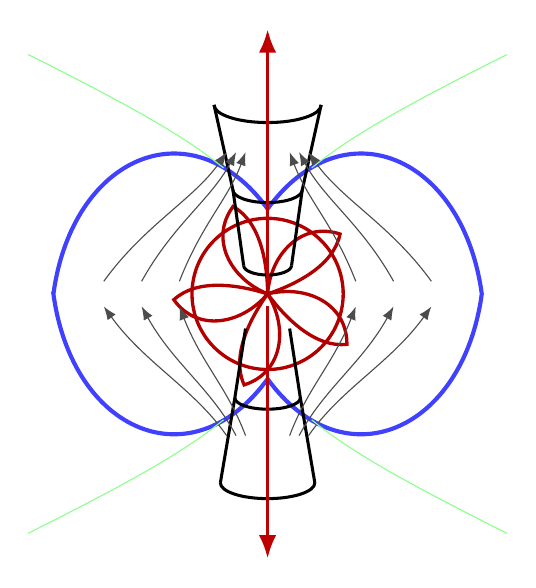
\begin{tikzpicture}[scale=0.8,>=Latex]
    % large toroidal lobes
    \draw[blue!75, line width=1.5pt]
      (-3.4,0) .. controls (-3.1,2.2) and (-1.2,3.0) .. (0,1.35)
      .. controls (1.2,3.0) and (3.1,2.2) .. (3.4,0)
      .. controls (3.1,-2.2) and (1.2,-3.0) .. (0,-1.35)
      .. controls (-1.2,-3.0) and (-3.1,-2.2) .. cycle;

    % inner red torus
    \foreach \a in {0,72,144,216,288}{
      \begin{scope}[rotate=\a]
        \draw[red!70!black, line width=1.2pt]
          (0,0) .. controls (0.45,0.15) and (1.05,0.45) .. (1.15,0.95)
          .. controls (0.55,1.15) and (0.05,0.65) .. (0,0);
      \end{scope}
    }
    \draw[red!70!black, line width=1.2pt] (0,0) circle (1.2);

    % axial funnel
    \draw[black, line width=1.1pt] (-0.85,3.0)--(-0.55,1.65)--(-0.38,0.45);
    \draw[black, line width=1.1pt] (0.85,3.0)--(0.55,1.65)--(0.38,0.45);
    \draw[black, line width=1.1pt] (-0.85,3.0) arc[start angle=180,end angle=360,x radius=0.85,y radius=0.28];
    \draw[black, line width=1.1pt] (-0.55,1.65) arc[start angle=180,end angle=360,x radius=0.55,y radius=0.2];
    \draw[black, line width=1.1pt] (-0.38,0.45) arc[start angle=180,end angle=360,x radius=0.38,y radius=0.15];

    \draw[black, line width=1.1pt] (-0.75,-3.0)--(-0.52,-1.65)--(-0.35,-0.55);
    \draw[black, line width=1.1pt] (0.75,-3.0)--(0.52,-1.65)--(0.35,-0.55);
    \draw[black, line width=1.1pt] (-0.75,-3.0) arc[start angle=180,end angle=360,x radius=0.75,y radius=0.25];
    \draw[black, line width=1.1pt] (-0.52,-1.65) arc[start angle=180,end angle=360,x radius=0.52,y radius=0.18];

    % field lines and arrows
    \foreach \x in {-2.6,-2.0,-1.4,1.4,2.0,2.6}{
       \draw[black!70, ->] (\x,0.2) .. controls ({0.75*\x},1.1) and ({0.45*\x},1.5) .. ({0.25*\x},2.25);
       \draw[black!70, ->] ({0.25*\x},-2.25) .. controls ({0.45*\x},-1.5) and ({0.75*\x},-1.1) .. (\x,-0.2);
    }

    % vertical red axis
    \draw[red!75!black, very thick, ->] (0,0.2) -- (0,4.2);
    \draw[red!75!black, very thick, ->] (0,-0.2) -- (0,-4.2);

    % faint external curves
    \draw[green!45] (-3.8,3.8) .. controls (-1.8,2.8) and (-1.2,2.4) .. (-0.7,2.0);
    \draw[green!45] (3.8,3.8) .. controls (1.8,2.8) and (1.2,2.4) .. (0.7,2.0);
    \draw[green!45] (-3.8,-3.8) .. controls (-1.8,-2.8) and (-1.2,-2.4) .. (-0.7,-2.0);
    \draw[green!45] (3.8,-3.8) .. controls (1.8,-2.8) and (1.2,-2.4) .. (0.7,-2.0);
\end{tikzpicture}
\end{center}

\uncertain{De rechterbladzijde bevat uitsluitend deze symmetrische torus-/velddoorsnede met een centrale vijfvoudige wervel en een verticale uitstroomas.}
\end{minipage}

\end{document}
